% Created 2023-09-15 Fri 20:04
% Intended LaTeX compiler: pdflatex
\documentclass[11pt]{article}
\usepackage[utf8]{inputenc}
\usepackage[T1]{fontenc}
\usepackage{graphicx}
\usepackage{longtable}
\usepackage{wrapfig}
\usepackage{rotating}
\usepackage[normalem]{ulem}
\usepackage{amsmath}
\usepackage{amssymb}
\usepackage{capt-of}
\usepackage{hyperref}
\author{Tim Hawes}
\date{\today}
\title{Characters}
\hypersetup{
 pdfauthor={Tim Hawes},
 pdftitle={Characters},
 pdfkeywords={},
 pdfsubject={},
 pdfcreator={Emacs 28.2 (Org mode 9.6.1)}, 
 pdflang={English}}
\begin{document}

\maketitle
\tableofcontents


\section*{Hallashim}
\label{sec:org0889d9d}
\subsection*{Faelinoril Galathil}
\label{sec:orgfac1739}

\begin{center}
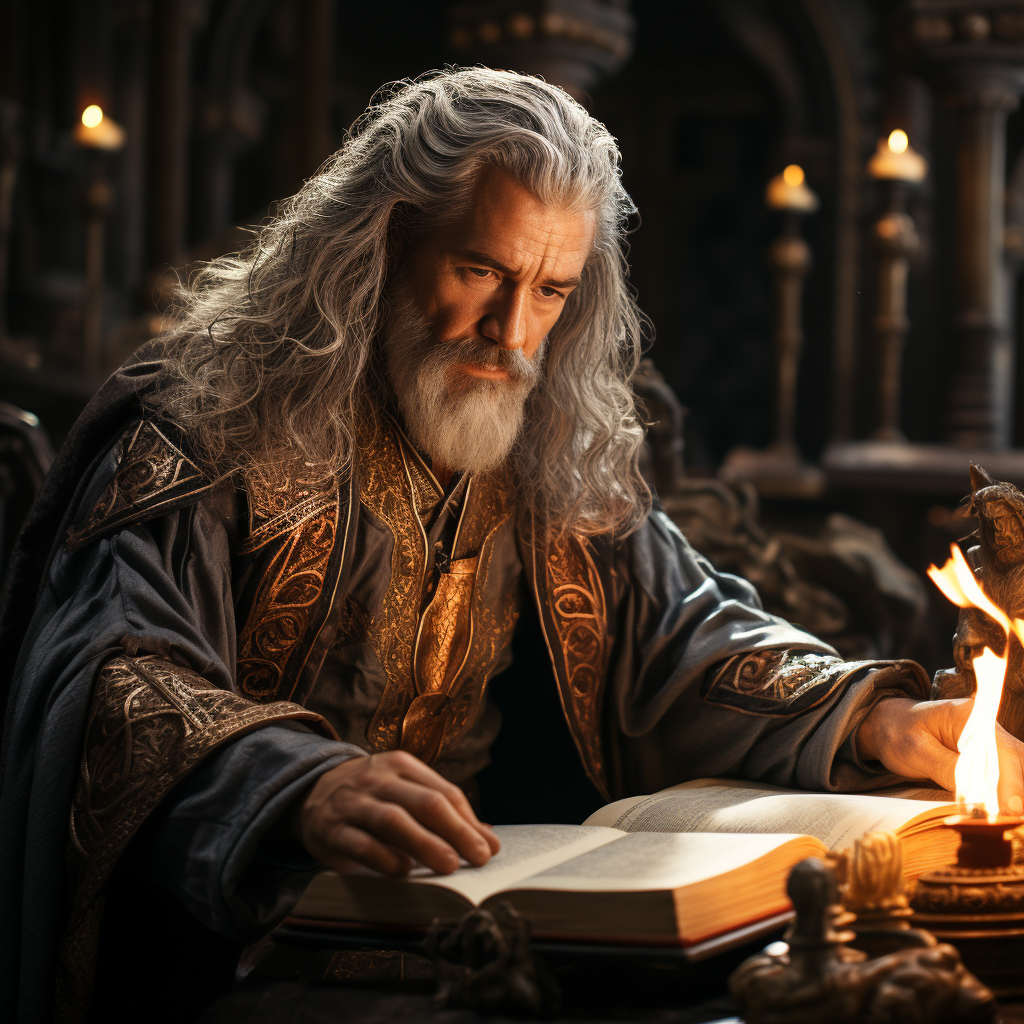
\includegraphics[width=500px]{./img/Faelinoril_Galathil.png}
\end{center}

\begin{description}
\item[{Age}] Elder (but not old)
\item[{Race}] Hallashim
\item[{Occupation}] Head Master of the Hallashim Archiver's Guild
\item[{Home}] Laurië Citime, in the city of Tanquende
\item[{Eneagram Scale}] Investigator
\item[{Background}] 
\end{description}
The second era Elves did lay traps throughout the Athalorion underground passages, to dissuade others from discovering their secrets.
The third era elves are generally not as stingy, but the riddles of Falasha's writings are as much a mystery to them as they are to others.
There is an old, wise Hallashim, by the name of Faelinoril Galathil. He is the headmaster of the Transcript guild at Laurië Citime. He has dedicated most of his life trying to unravel Falasha's encrypted words and the secrets burried in the Athalorian ruins.

Faelinoril's magnum ops, ``In Átaremma's Footsteps'', he reveals some the success the old elves had in translating enough of the Amearan tongue to form some simple phrases. He further was able to cross-reference these phrases in Falasha's poems. This was a huge breakthrough in the research of the Amearans.
\subsection*{Elarialaith Lóteiirimaeth}
\label{sec:orgab78807}

\begin{center}
\includegraphics[width=500px]{./img/Elarialaith_Lóteiirimaeth.png}
\end{center}

\begin{description}
\item[{Age}] Young Adult
\item[{Race}] Hallashim
\item[{Occupation}] Journeyshim in the Hallashim Archiver's Guild
\item[{Home}] Laurië Citime, in the city of Tanquende
\item[{Eneagram Scale}] Reformer
\end{description}

\section*{Palaman}
\label{sec:org2de3407}
\subsection*{Tadhg MacMurchadha}
\label{sec:org55bc645}

\begin{center}

\includegraphics[width=500px]{./img/Tadhg_MacMurchadha.png}
\end{center}

\begin{description}
\item[{Age}] Young Adult
\item[{Race}] Palaman
\item[{Occupation}] Scholar in Ponte Cidade
\item[{Home}] Ponte Cidade
\item[{Eneagram Scale}] Investigator
\end{description}
\section*{Other}
\label{sec:org814c882}
\subsection*{Ryu Angus}
\label{sec:org85082f9}

\begin{center}

\includegraphics[width=500px]{./img/Ryu_Angus.png}
\end{center}

\begin{description}
\item[{Age}] Young Adult
\item[{Race}] Palaman
\item[{Occupation}] Undetermined
\item[{Home}] Ponet Cidade??
\item[{Eneagram Scale}] The Challenger
\end{description}
\end{document}